\chapter{Vision System}\label{ch:hardware}
\raggedbottom
This research is focused on the development of an image processing algorithm able to detect deposition geometry in a robust manner. By robust is meant that the algorithm should still be able to detect the right geometry under sub-optimal image conditions. The images the algorithm processes are generated by the vision system hardware. To test robustness a vision system has been selected consisting out of low-quality components.  

The vision system hardware setup is discussed in this chapter. First, an overview is given of all the elements in the vision system. Then the different triangulation configurations are discussed. Next, the major components are further explained and at last the generated output is analyzed. 

\section{Overview}

A general overview of the components of the experimental setup is shown in Figure \ref{fig:setup_overview}. The vision system consists out of a camera and a laser which are fixed in position by a mount bracket. This bracket is attached to the AM machine. The laser exposes the geometry of the line deposited on the bed. The camera is connected to the laptop and the software runs the image processing algorithm on the images from the camera detecting the geometry of the depositions.
\skippar
\begin{figure}[!ht]
   \centering
   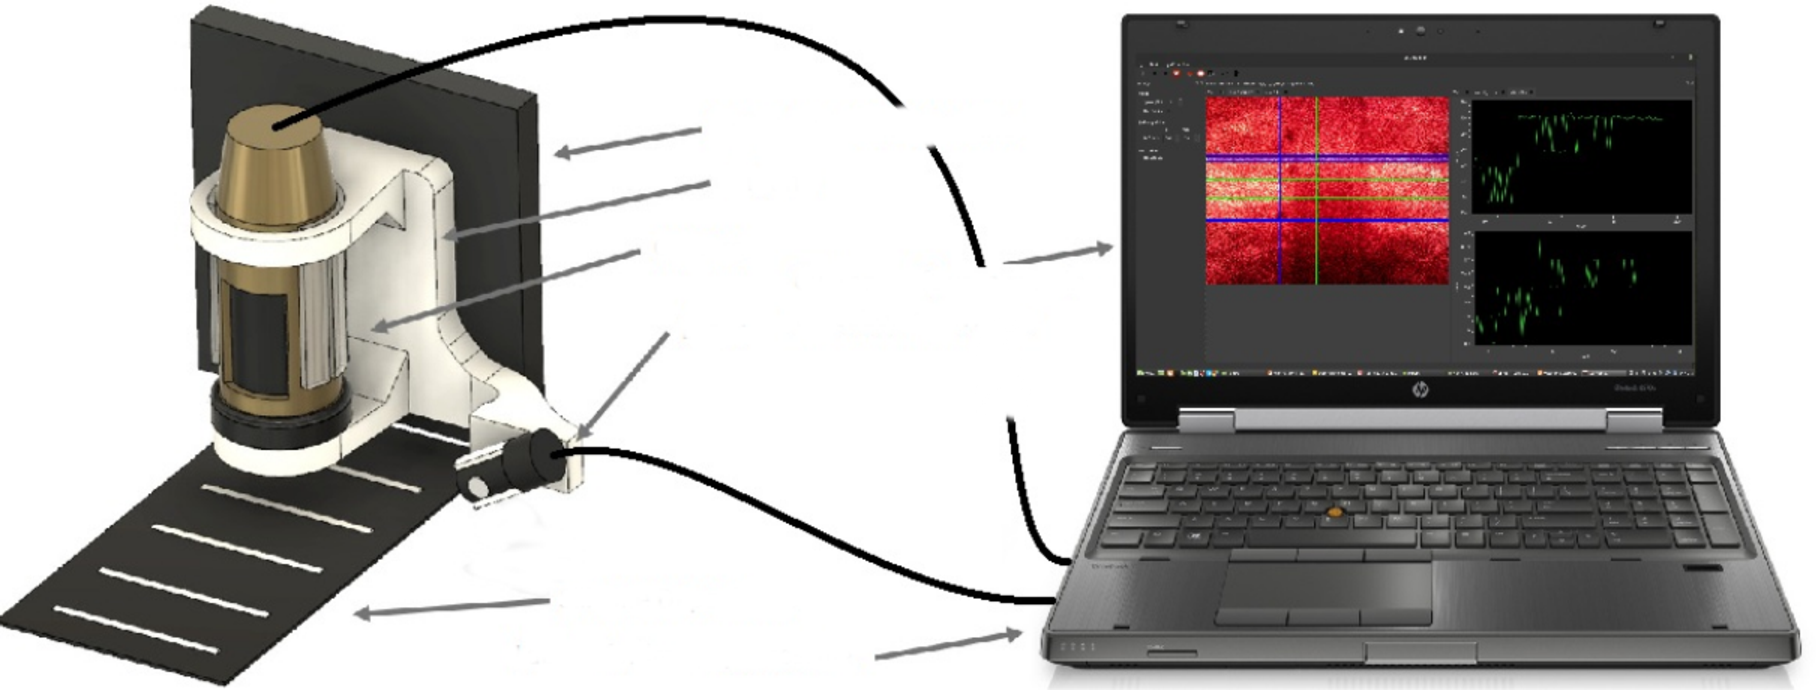
\includegraphics[width=\textwidth]{setup_overview.pdf}
   \setlength{\unitlength}{0.1\textwidth}
   \footnotesize\put(-6.1,3.03){AM machine}
   \footnotesize\put(-6,2.75){Mount}
   \footnotesize\put(-6.4,2.35){Camera}
   \footnotesize\put(-6.4,2){Laser}
   \footnotesize\put(-6.9,0.4){Deposited material}
   \footnotesize\put(-8,0.1){Laptop for image processing}
   \footnotesize\put(-5.6,2.1){Custom software}
   \footnotesize\put(-5.6,1.9){running detection}
   \footnotesize\put(-5.6,1.7){algorithm}
   \caption{Overview of vision system components. }
   \label{fig:setup_overview}
\end{figure}
\skippar
An overview of the vision system in reality is shown in Figure \ref{fig:setup_real}. The laser emits a red colored line which illuminates the deposited material. The laser line quality is low as shown by the noise around the center of the line. The line follows the geometry of the deposition exposing the profile to the camera. The deposition lines are printed and UV-cured as described in \cite{vlasea2013experimental}.
\begin{figure}[!ht]
   \centering
   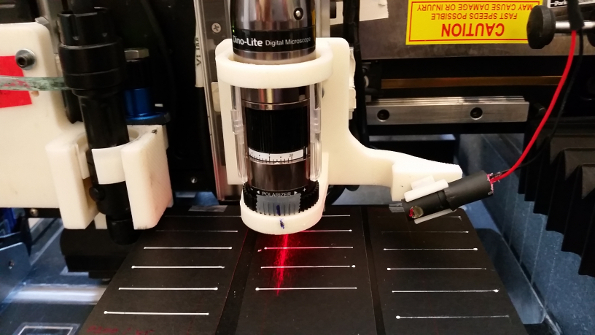
\includegraphics[width=0.65\textwidth]{setup_real.jpg}
   \setlength{\unitlength}{0.1\textwidth}
   \thicklines
   {\color{brown}\put(-7,3.3){\vector(3,-1){3.4}}}
   \footnotesize\put(-7.85,3.25){Camera}
   {\color{brown}\put(-7,2){\vector(3,-1){3.4}}}
   \footnotesize\put(-8,2){Laser line}
   {\color{brown}\put(-7,1){\vector(3,-1){2.3}}}
   \footnotesize\put(-8.05,1){Deposited}
   \footnotesize\put(-8.05,0.8){material}
   {\color{brown}\put(0.15,3.5){\vector(-3,-1){3.1}}}
   \footnotesize\put(0.2,3.45){Mount}
   {\color{brown}\put(0.15,2.2){\vector(-3,-1){1.65}}}
   \footnotesize\put(0.2,2.15){Laser}
   {\color{brown}\put(0.15,2.2){\vector(-3,-1){1.00}}}
   \footnotesize\put(0.2,3.45){Laser line}
   \caption{Overview of vision system in reality.}
   \label{fig:setup_real}
\end{figure}

\section{Triangulation Configuration}

A triangulation based configuration is used for the measurement of the deposition geometry. This configuration consists out of a line-laser and a camera placed at a relative angle to each other. The line emitted by the laser illuminates the material in its path. A different angle of the camera relative to the laser is needed to expose the geometry of the illuminated material. Images created by the camera are generally thought to look as displayed in Figure \ref{fig:profile}. The angular placement of the components with respect to each other and the bed has consequences for the quality of the images created. Four commonly used configuration setups are shown in Figure \ref{fig:triangulations} and the side view of the reverse configuration in Figure \ref{fig:reverse}.

\begin{figure}[!ht]
\begin{subfigure}{0.69\textwidth}
\centering
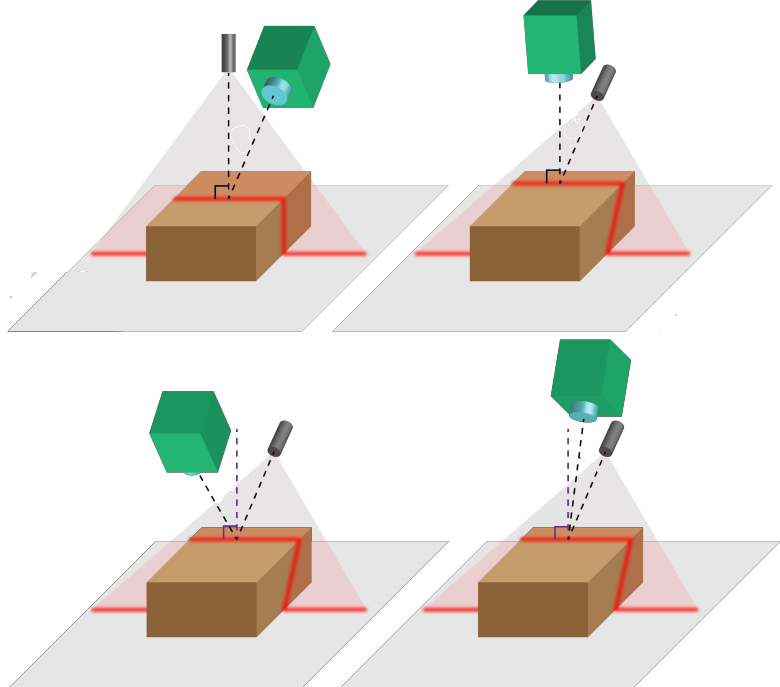
\includegraphics[width=1\linewidth]{laser_triangulation} 
\setlength{\unitlength}{0.1\textwidth}
\footnotesize\put(-9.2,4.7){Standard}
\footnotesize\put(-5,4.7){Reverse}
\footnotesize\put(-9.2,0.1){Specular}
\footnotesize\put(-5,0.1){Look-Away}
\caption{Four common triangulation configurations.}
\label{fig:triangulations}
\end{subfigure}
\begin{subfigure}{0.295\textwidth}
\centering
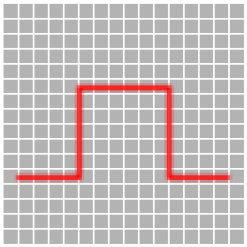
\includegraphics[width=1\linewidth]{profile}
\caption{Camera View}
\label{fig:profile}
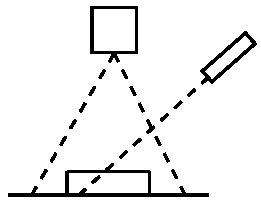
\includegraphics[width=1\linewidth]{triangulation}
\caption{Reverse side-view}
\label{fig:reverse}
\end{subfigure}
\caption{Laser Line Triangulation}
\end{figure}
\skippar
Each configuration has advantages and disadvantages. Important factors to consider when choosing a configuration are:
\paragraph{Resolution} Placing the laser at a shallow angle with respect to the bed, and the camera at $90$ degrees relative to the laser is optimal for a large height resolution. The camera view as shown in Figure \ref{fig:profile} would show a large line height. This is advantages for the measurement of height from the image. 

\paragraph{Focus} Placing the camera at a shallow angle with respect to the bed will result in focus loss. Only a very narrow point on the deposition will be focused. The camera at $90$ degrees will be able to focus on the whole field of view and the best pixel/inch ratio. At this point the least amount of deposition area is converted to the largest amount of pixels. The shallower the angle, the lower the ratio. 

\paragraph{Line Spreading} Placing the laser a a shallow angle spreads the line out over a larger area compared to an angle of $90$ degrees relative to the bed. The line will therefore loose brightness.

\paragraph{Dimensions} Large components have to be placed further away. Small components can be placed very close which could influence other factors.

\paragraph{Inclusion} A shallow angle for the camera or laser will result in material inclusion. The camera or laser will not be able to illuminate or observe a certain area of the material.

\paragraph{Reflection} Certain angles between the camera and the laser will result in reflection. The laser could saturate the image and pixel difference would be lost.

\skippar
Using the above factors the four common configurations are ranked. Table \ref{tab:triangulation_rank} shows the score of each configuration at each factor.
\begin{table}[ht]
\centering
\begin{tabular}{lllll} \hline 
Configuration & Standard & Reverse & Specular & Look-Away \\
\hline
Resolution & + & ++ & +++ & - \\
Focus & - & +++ & + & ++ \\
Line Spreading & +++ & - & ++ & + \\
Dimensions & + & ++ & +++ & - \\
Inclusion & ++ & + & - & +++ \\
Reflection & ++ & + & - & +++ \\
\hline
Score & 8 & 8 & 7 & 7 \\
\hline
\end{tabular}
\caption{Triangulation Configuration Rankings.}
\label{tab:triangulation_rank}
\end{table}
\skippar
The Standard and Reverse configuration score best. Each configuration has however its own application domain where some factors are preferable over others. The application of each configuration is discussed as follows:

\paragraph{Standard} Maximal reduction of line width through the placement of the laser at the top. Very sharp laser line as long as there are not large height differences in the material to be observed. To gain resolution the camera should be placed at a shallow angle at the cost of camera focus. A shallow angle also introduces inclusion problems and could lead to reflection.

\paragraph{Reverse} Perfect focus of the camera on the whole field of view. If the material has large height differences this is however compromised.  The laser angle has the same properties as the Standard configuration. 

\paragraph{Specular} The camera and the laser at a $90$ degree angle relative to each other for perfect resolution. Reflection could however introduce problems. Focus and line spreading are also not optimal.

\paragraph{Look-Away} Best possible reduction of inclusion and reflection. Very bad resolution.

\skippar
Our application is on the printing of deposition lines to build parts for additive manufacturing. The lines printed should eventually be controlled to have a constant geometry at all times. Our configuration should be focused on the ability to measure as accurately as possible. A constant surface is extra beneficial for the camera to focus on the entire field of view. Therefore the \textbf{Reverse configuration is chosen} as the setup for the vision system.

\section{Camera}

% Quality aspects of cameras
The camera ultimately determines the performance of the system. The performance of the algorithm designed to process images relies on the quality and amount of data per unit of movement of the deposition. Image quality is affected by camera resolution and the amount of data per pixel. A high resolution with a high range of possible values for each pixel amount for maximum variability and best image quality. The amount of data per unit is affected by the optical zoom and the frame rate of the camera. A large optical zoom results in a high amount of pixels per area. A high frame rate results in more measurements. 

% our camera and its specifications
Low-cost cameras compromise on the above quality aspects. The camera used for this research is a Dino-Lite Camera as shown in Figure \ref{fig:camera}. Important specifications are given in Table \ref{tab:cam_specs}. 

{\centering \vspace*{\baselineskip}
\begin{minipage}{0.45\textwidth}
   \centering
   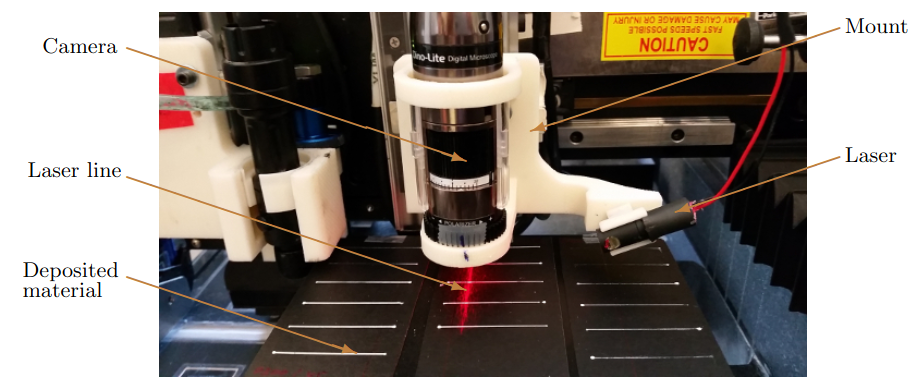
\includegraphics[width=1\textwidth]{dinolite} 
   \label{fig:camera}
   \captionof{figure}{Dino-Lite Camera}
\end{minipage}
\begin{minipage}{0.58\textwidth}
   \centering
    \begin{tabular}{ll}\hline \hline
		Model & AM7515MZTL Edge  \\
		Interface & USB 2.0 \\
		Resolution & 5MP (2592x1944) \\
		Frame Rate & 10fps @ 5MP \\
		Pixel & 3-Channel 8-bit RGB \\
		Magnification & 10x - 140x Optical \\
		Dimension & 10.5cm (H) x 3.2cm (D) \\ \hline
	\end{tabular}
	\label{tab:cam_specs}
    \captionof{table}{Dino-Lite Specifications}
\end{minipage}
}

% Our camera analysis
\skippar
The Dino-Lite produces 5 Mega-pixel images at a maximum frame rate of 10 frames per second. The optical zoom is 140 times which makes up for the lower resolution in terms of pixels per area. The frame rate is very low and use for \textbf{real-time control is not recommended with this camera.} The camera could miss a corner and which is unacceptable for control purposes. The quality of the images is however good and the camera is therefore perfectly applicable to measure depositions if time is not a constraint. Off-line use to measure the deposition is possible. Identifying dynamics is hard due to the lack of timed data. \textbf{Steady-state modeling is however possible.}
\begin{table}[!ht]
\centering
\begin{tabular}{ll} \hline \hline
Pixels/Image & $2.592 * 1.944 = 5.038.848$  \\
Integers/Image & $2.592 * 1.944 * 3 = 15.116.544$\\
MB/Image & $\approx15$ \\ 
Possible Values/Pixel & $256^3 = 16.777.216$\\ \hline
\end{tabular}
\caption{ Dino-Lite camera data output.}
\label{tab:camera_output}
\end{table}% talk about the amount of data and the consequences for the image processing and hardware
\skippar
The amount of data the camera produces is given in Table \ref{tab:camera_output}. This amount of data needs however to be processed by the detection algorithm. Expensive hardware and optimized software make it possible to process the data fast. Implementing complex detection algorithms compromise the speed of execution but could improve accuracy of measurement. Simpler algorithms tend to be fast but not as accurate. There has to be found a balance between speed and accuracy of the algorithm. For real-time control purposes high sampling rates could be preferred over super accurate measurement. Furthermore, complex indeterministic algorithms introduce jitter in the sampling rate, which is highly undesirable in control. Since the ultimate goal is real-time control of the deposition geometry \textbf{this research focuses on the development of a detection algorithm utilizing simple deterministic image processing methods.} 

\section{Laser-Diode}
% Quality aspects of laser
The laser is used for illumination of the geometry of the object being detected. The lens within the laser converts the dot shaped light to a line. This line has a width which should be relatively small compared to the field of view of the camera. The line could have different intensity profiles.  A linear profile has equal intensity along the line. Gaussian lines have intensity according to a Gaussian profile, meaning high intensity in the middle and lower at the ends. The output power of the laser is another indicator for overall intensity of the light the laser emits. Different wavelengths produce different colors and have their own advantages with respect to visibility on certain surfaces. 

{\centering \vspace*{\baselineskip}
\begin{minipage}{0.49\textwidth}
   \centering
   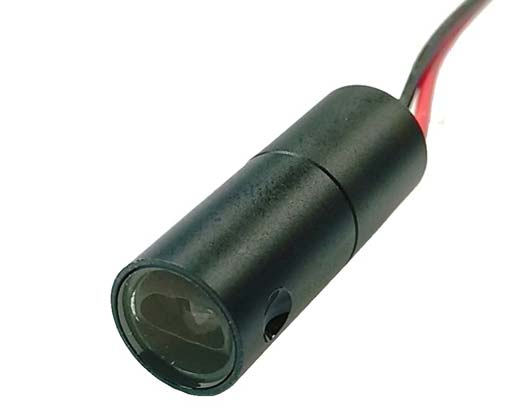
\includegraphics[width=0.8\textwidth]{laser} 
   \label{fig:laser}
   \captionof{figure}{Infiniter Line-Laser}
\end{minipage}
\begin{minipage}{0.49\textwidth}
   \centering
\begin{tabular}{ll} \hline \hline
Model & VLM-650-30  \\
Interface & Lead Wires \\
Operating Voltage & 5 Volt \\
Output Power & 5mW \\
Wavelength & 650 nm \\
Fan Angle & 60 degree \\
Line Profile & Gaussian Line \\
Line Thinness & $<$ 1.2mm \\
Accuracy & $<$1.6mm @ 400mm \\ \hline
\end{tabular}
\captionof{table}{Laser Specifications.}
\label{tab:laser_specs}
\end{minipage}
}

\skippar
% our laser and its specifications
Low-cost line-lasers compromise on the above quality aspects. The laser used for this research is a Infiniter line laser as shown in Figure \ref{fig:laser}. Important specifications are given in Table \ref{tab:laser_specs}. 

% Our laser analysis
The laser produces red light at 650nm and the output power is 5mW. The output power is low and there are no safety restrictions. The line is relatively thick which only allows for proportional large field of view and therefore might restrict the amount of optical zoom used. 

\section{Deposition Material}
% reflection, absorption, transparancy
The material used for printing has a big influence on the image quality produced by the camera. Light reflection can cause pixel saturation which makes detecting differences between the pixels hard or even impossible. Absorption leads to the same problem implied by the lack of light. A material that does not reflect or absorb and passes through makes it impossible to detect differences between the bed and the object to be detected. 
\begin{figure}[!ht]
\begin{subfigure}{0.32\textwidth}
\centering
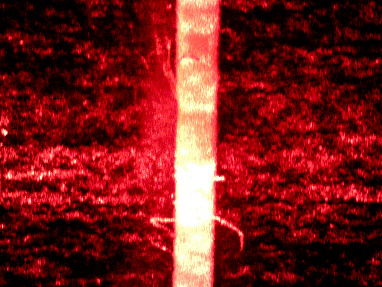
\includegraphics[width=1\linewidth]{white} 
\caption{White Silicon}
\label{fig:white}
\end{subfigure}
\begin{subfigure}{0.33\textwidth}
\centering
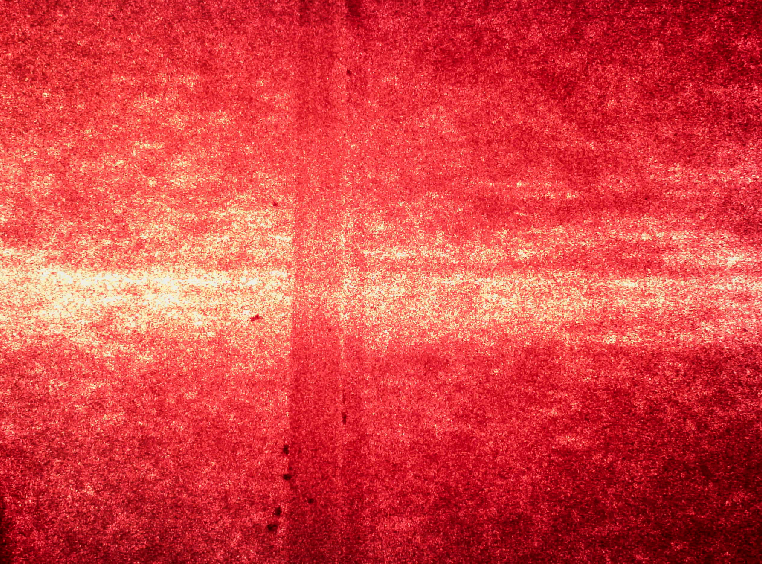
\includegraphics[width=1\linewidth]{silicon}
\caption{Transparent Silicon}
\label{fig:transparant}
\end{subfigure}
\begin{subfigure}{0.33\textwidth}
\centering
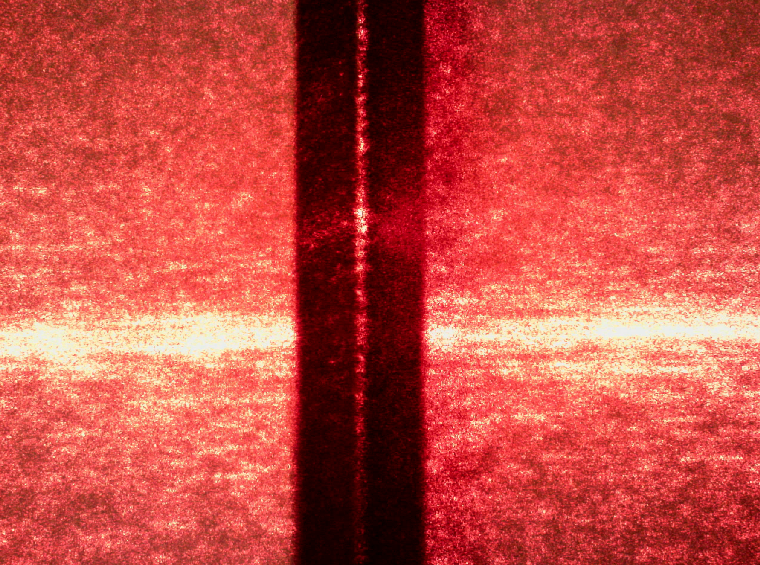
\includegraphics[width=1\linewidth]{inbus}
\caption{Black Rod}
\label{fig:black}
\end{subfigure}
\caption{Camera view for different types of deposition material.}
\label{fig:material}
\end{figure}
% Talk about figures
\skippar
Figure \ref{fig:material} shows the images acquired for different materials. Figure \ref{fig:white} shows a white silicon based deposition material which is highly reflective. Contrast between the bed and the deposition is high but saturation of pixels occurs on top of the deposition. Figure \ref{fig:transparent} shows the result for a transparent silicon. Pixels do not saturate but contrast is low. Figure \ref{fig:black}  shows the image when a black rod is used for material. This rod absorbs most of the light and the laser line does not expose the geometry of the rod. 

% talk about chosen material and why
Due to the reasons explained above this research is focused on the usage of \textbf{white silicon as the deposition material.} The reflection of the material is a disadvantage but could also be the result when a different triangulation configuration was used like the Specular configuration as can be seen in Figure \ref{fig:triangulations}. Transparency and absorption make measurement through a triangulation based setup very hard.
